\section{Введение}
\begin{frame}
    \frametitle{Сферы высказываний}
    \begin{columns}
        \begin{column}{0.5\textwidth}
            В аксиоматике социологии выделяют различные автономные сферы
            человеческого действия по принципам:
            \begin{itemize}[<+->]
                \item Свой язык
                \item Своя логика
                \item Своя рациональность
                \item Свой способ производства высказываний и действий
            \end{itemize}
        \end{column}
        \begin{column}{0.5\textwidth}
            Замкнутые системы согласно этой аксиоматике:
            \begin{itemize}[<+->]
                \item Философия
                \item Религия
                \item Искусство
                \item Политика
                \item Наука
                \item Право
                \item Хозяйствование
                \item Быт
            \end{itemize}
        \end{column}
    \end{columns}
\end{frame}

\begin{frame}
    \frametitle{Замкнутые системы}
    \only<1->{
        Философия: познание наиболее базовых принципов изучения мира, человека,
        и отношений между людьми
    }
    \only<2->{
        \par\vspace{0.3cm}
        Религия (обычно): отношение к непознаваемому
    }
    \par\vspace{0.3cm}
    \only<3->{
        Искусство: образное осмысление действительности
    }
    \only<4->{
        \par\vspace{0.3cm}
        Политика: совершение активных действий для изменения или консервации
        текущего положения дел
    }
    \only<5->{
        \par\vspace{0.3cm}
        Наука: познание мира
    }
\end{frame}


\begin{frame}
    \frametitle{Наука}
    \only<1->{
        \par\vspace{0.3cm}
        Математика: наука об отношениях между формальными объектами
    }
    \only<2->{
        \par\vspace{0.3cm}
        Лингвистика: наука о языках
    }
    \only<3->{
        \par\vspace{0.3cm}
        Социология: наука об отношениях между группами людей
    }
    \only<4->{
        \par\vspace{0.3cm}
        Психология: наука о психической деятельности людей и
        групп людей
    }
    \only<5->{
        \par\vspace{0.3cm}
        Химия: наука о веществе на молекулярном уровне
    }
    \only<6->{
        \par\vspace{0.3cm}
        Биология: наука о живой материи
    }
    \only<7->{
        \par\vspace{0.3cm}
        Музыкознание: наука о музыке
    }
\end{frame}

\begin{frame}
    \frametitle{Физика как наука о фундаментальных законах материи}
    Историческое развитие физики
    \begin{itemize}[<+->]
        \item Аристотель (IV век до н.э.): формулирует всеобщие законы
            движения, космологии, химии, биологии, и т.д.
        \item Галилей (XVII век): законы движения и экспериментальный
            метод
        \item Ньютон (XVII--XVIII): механика, математический анализ
        \item Кельвин, Больцман (XIX век): термодинамика и
            статистическая физика
        \item Фарадей и Максвелл (XIX век): электричество и магнетизм
        \item Эйнштейн (XX век): общая теория относительности
        \item Планк, Борн (XX век): квантовая механика
        \item Салам, Вайнберг (XX век): электрослабая теория
    \end{itemize}
\end{frame}
\begin{frame}
    \frametitle{Физика как наука о фундаментальных законах материи}
    Современные разделы физики:
    \begin{itemize}[<+->]
        \item Физика элементарных частиц
        \item Астрофизика
        \item Космология
        \item Атомная физика
        \item Квантовая оптика
        \item Физика плазмы
        \item Химическая физика
        \item Биофизика
    \end{itemize}
\end{frame}

\begin{frame}
    \frametitle{Карьера в физике}
    \only<1->{
        \par\vspace{0.3cm}
        Школа
    }
    \only<2->{
        \par\vspace{0.3cm}
        Бакалавриат (1--2 курсы)
    }
    \only<3->{
        \par\vspace{0.3cm}
        Выбор кафедры, бакалавриат (3--4 курсы)
    }
    \only<4->{
        \par\vspace{0.3cm}
        Магистратура (5--6 курсы)
    }
    \only<5->{
        \par\vspace{0.3cm}
        Аспирантура (от трёх лет до бесконечности)
    }
    \only<6->{
        \par\vspace{0.3cm}
        Post-doctoral research (рабочие лошидки науки)
    }
    \only<7->{
        \par\vspace{0.3cm}
        Профессура (боги науки)
    }
\end{frame}

\begin{frame}
    \begin{figure}
        \begin{centering}
            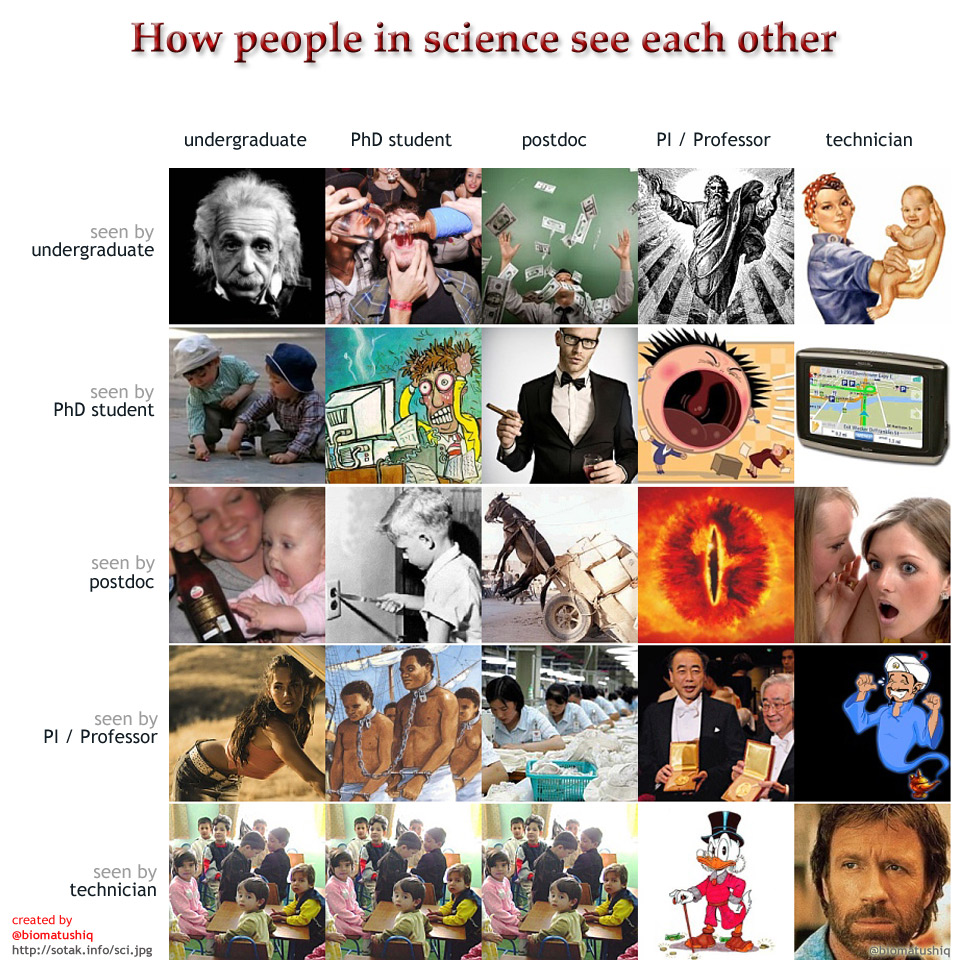
\includegraphics[width=0.6\textwidth]{sci}
        \end{centering}
    \end{figure}
\end{frame}
